%!TEX root=main.tex
\section{架构}
\label{clicknp:sec:architecture}

\subsection{系统架构}
\label{clicknp:subsec:sysarch}

图 \ref{clicknp:fig:clicknp} 显示了 \name 的体系结构。
\name 以 Catapult Shell 架构构 建\cite {putnam2014reconfigurable}。
\textit {shell}包含许多可重用的逻辑位,这些逻辑对所有应用程序都是通用的,并将它们抽象为一组明确定义的接口,例如,PCIe,直接内存访问(DMA),DRAM内存管理单元(MMU),和以太网MAC。
\name FPGA程序合成为 Catapult \textit {用户逻辑}。
但是,由于\name 依赖于商品高层次综合工具链来生成FPGA 硬件描述语言,并且不同的工具可以为shell管理的资源生成自己的(和不同的)接口,需要一个\textit {高层次综合的特定运行时}(Board Specific Package,BSP),用于执行高层次综合特定接口与shell接口之间的转换。


\begin{figure}
	\centering
	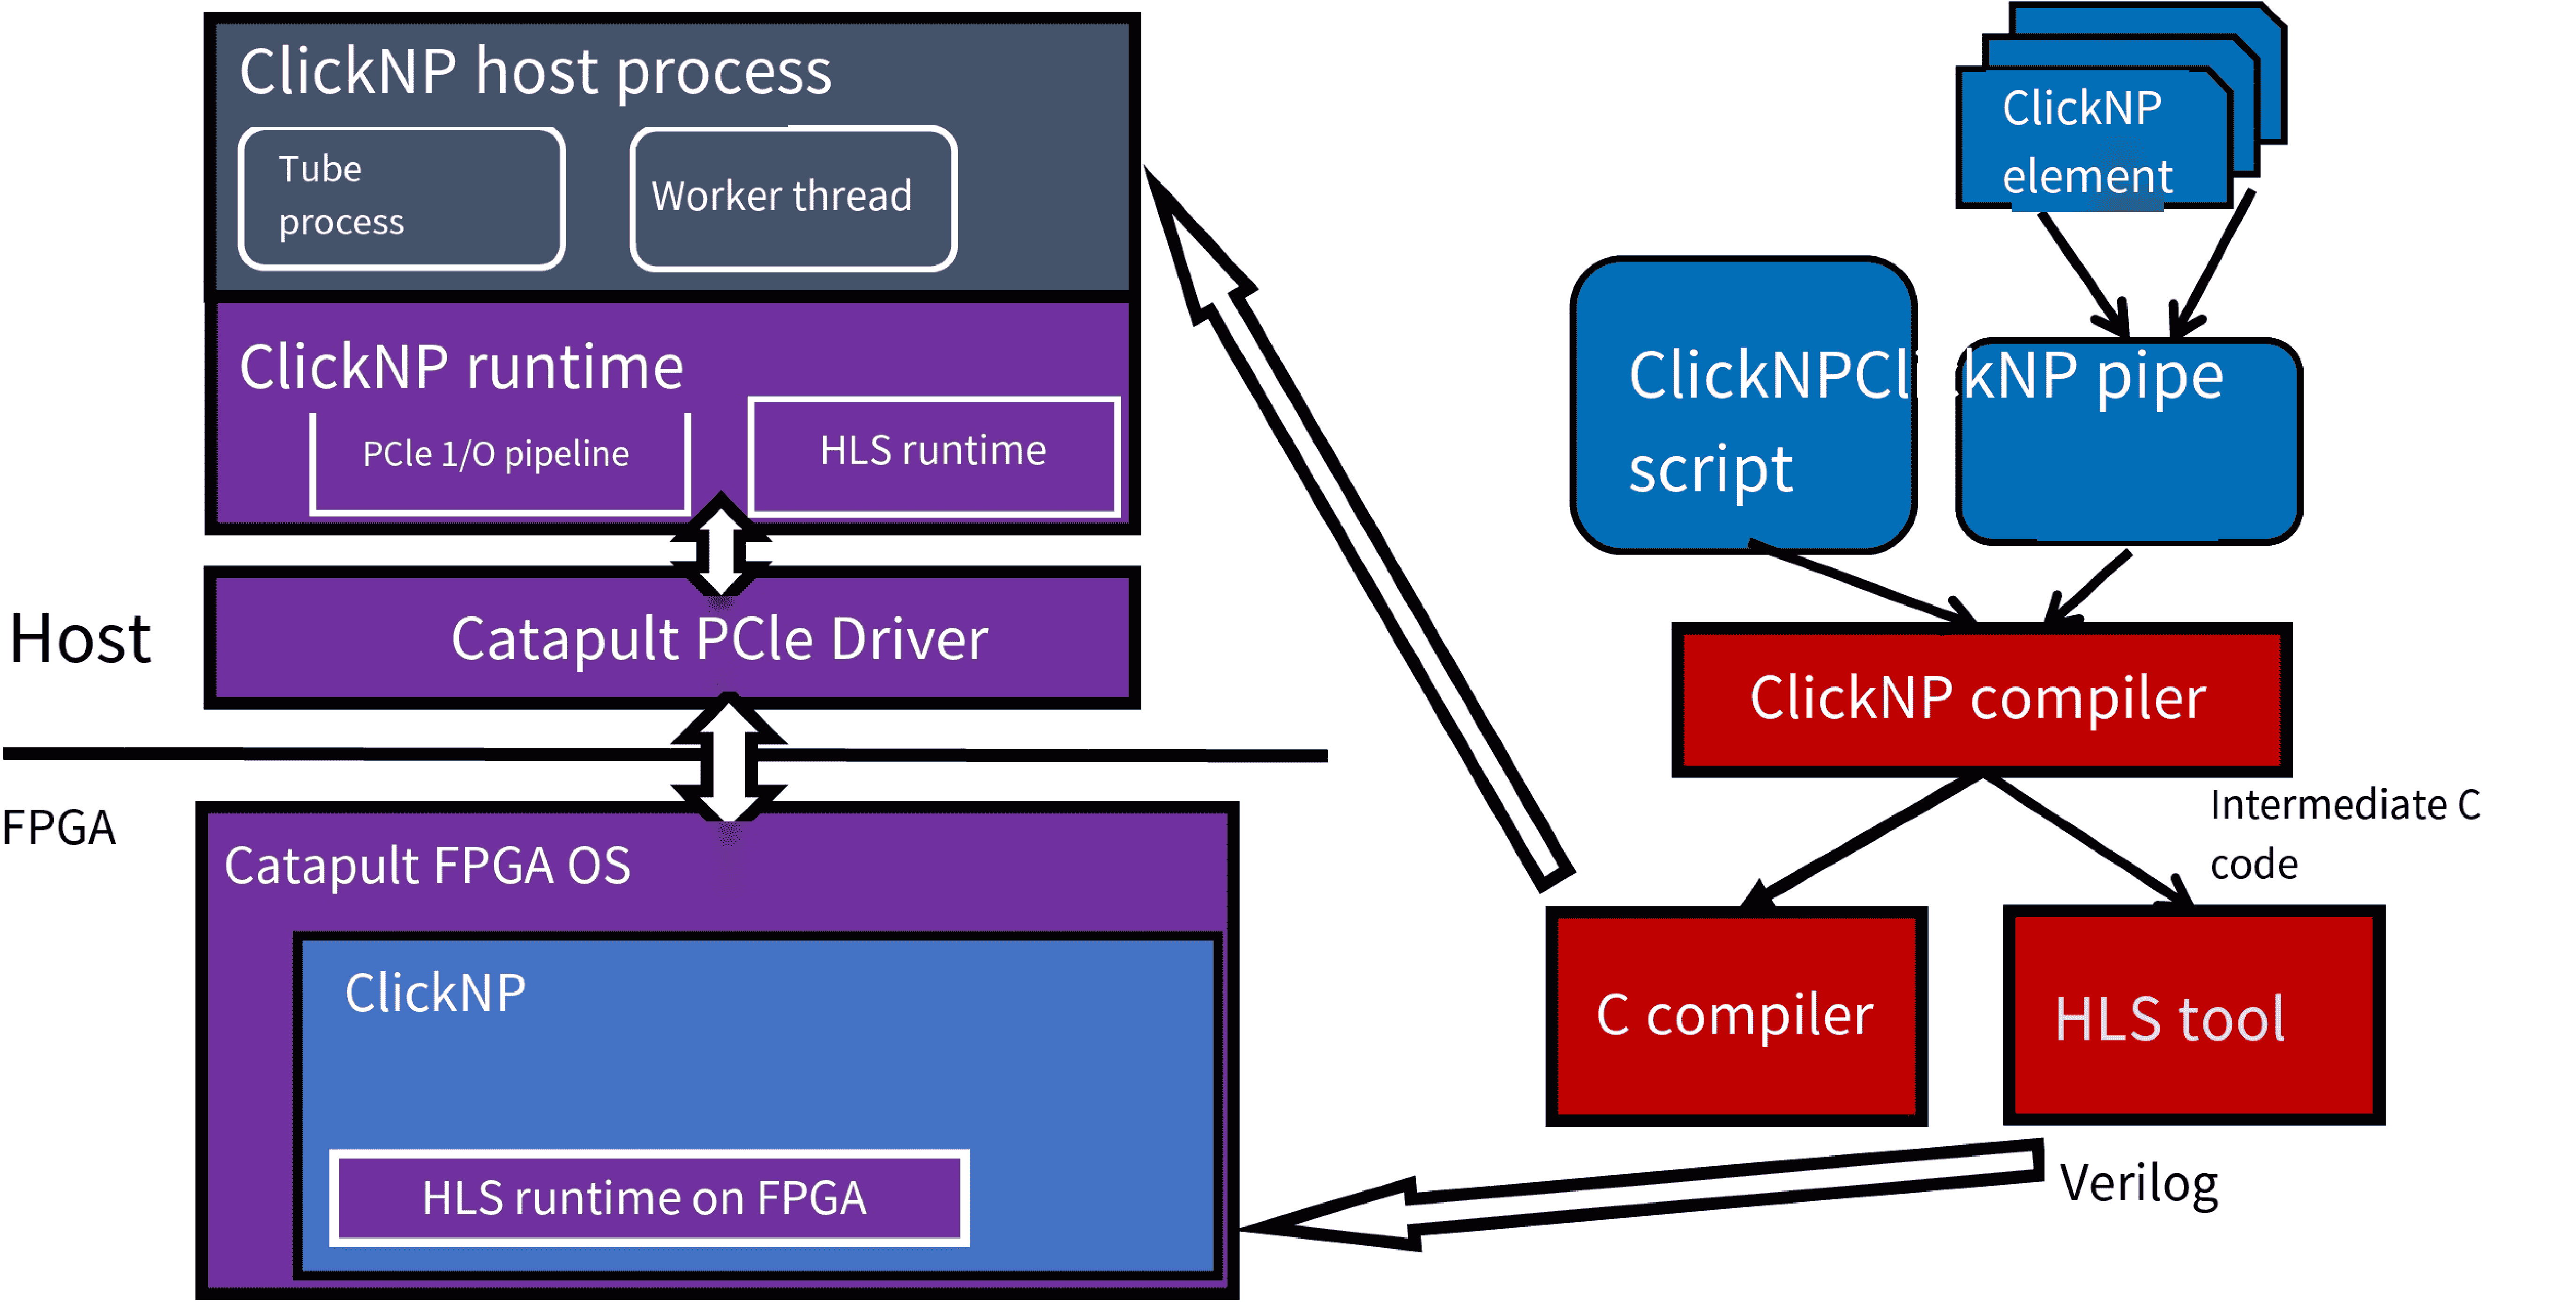
\includegraphics[width=.8\textwidth]{clicknp_arch.pdf}
	\caption{ClickNP 架构。}
	\label{clicknp:fig:clicknp}
\end{figure}


\name{} 主机(host)进程通过 \name{} 运行库与 \name{} 用户逻辑进行通信,这进一步依赖于 Catapult PCIe 驱动程序中的服务与FPGA硬件进行交互。
\name{} 运行库实现了两个重要的功能:
(1)它暴露了一个PCIe通道API,以实现 \name{} host进程和角色之间的高速和低延迟通信;
(2)它调用几个高层次综合特定库将初始参数传递给角色中的模块,并控制这些模块的启动/停止/复位。
\name{} 主机进程有一个管理器线程和零个或多个工作线程。
管理器线程将FPGA映像加载到硬件中,启动工作线程,根据配置初始化FPGA和CPU中的\name 元件,并通过在运行时向元件发送\textit {信号}(signal)来控制它们的行为。
如果将每个工作线程分配给CPU,则每个工作线程可以处理一个或多个模块。

\subsection{\name 编程}

\subsubsection{抽象}

\name 提供模块化架构,基本处理模块称为\textit{元件}(element)。
如图 \ref{clicknp:fig:element_arch} 所示,\name 元件具有以下属性:
\begin{itemize}
\item 本地状态。 每个元件都可以定义一组只能在元件内部访问的局部变量。
\item 输入和输出端口。 元件可以具有任意数量的输入或输出端口。
\item 处理程序功能。 元件有三个处理函数:(1)初始化处理程序,在元件启动时调用一次,(2)处理处理程序,连续调用以检查输入端口和处理可用数据,以及(3)信号处理程序 ,它从主机程序中的管理器线程接收和处理命令(\textit {信号})。
\end{itemize}

\begin{figure}[htbp]
\centering
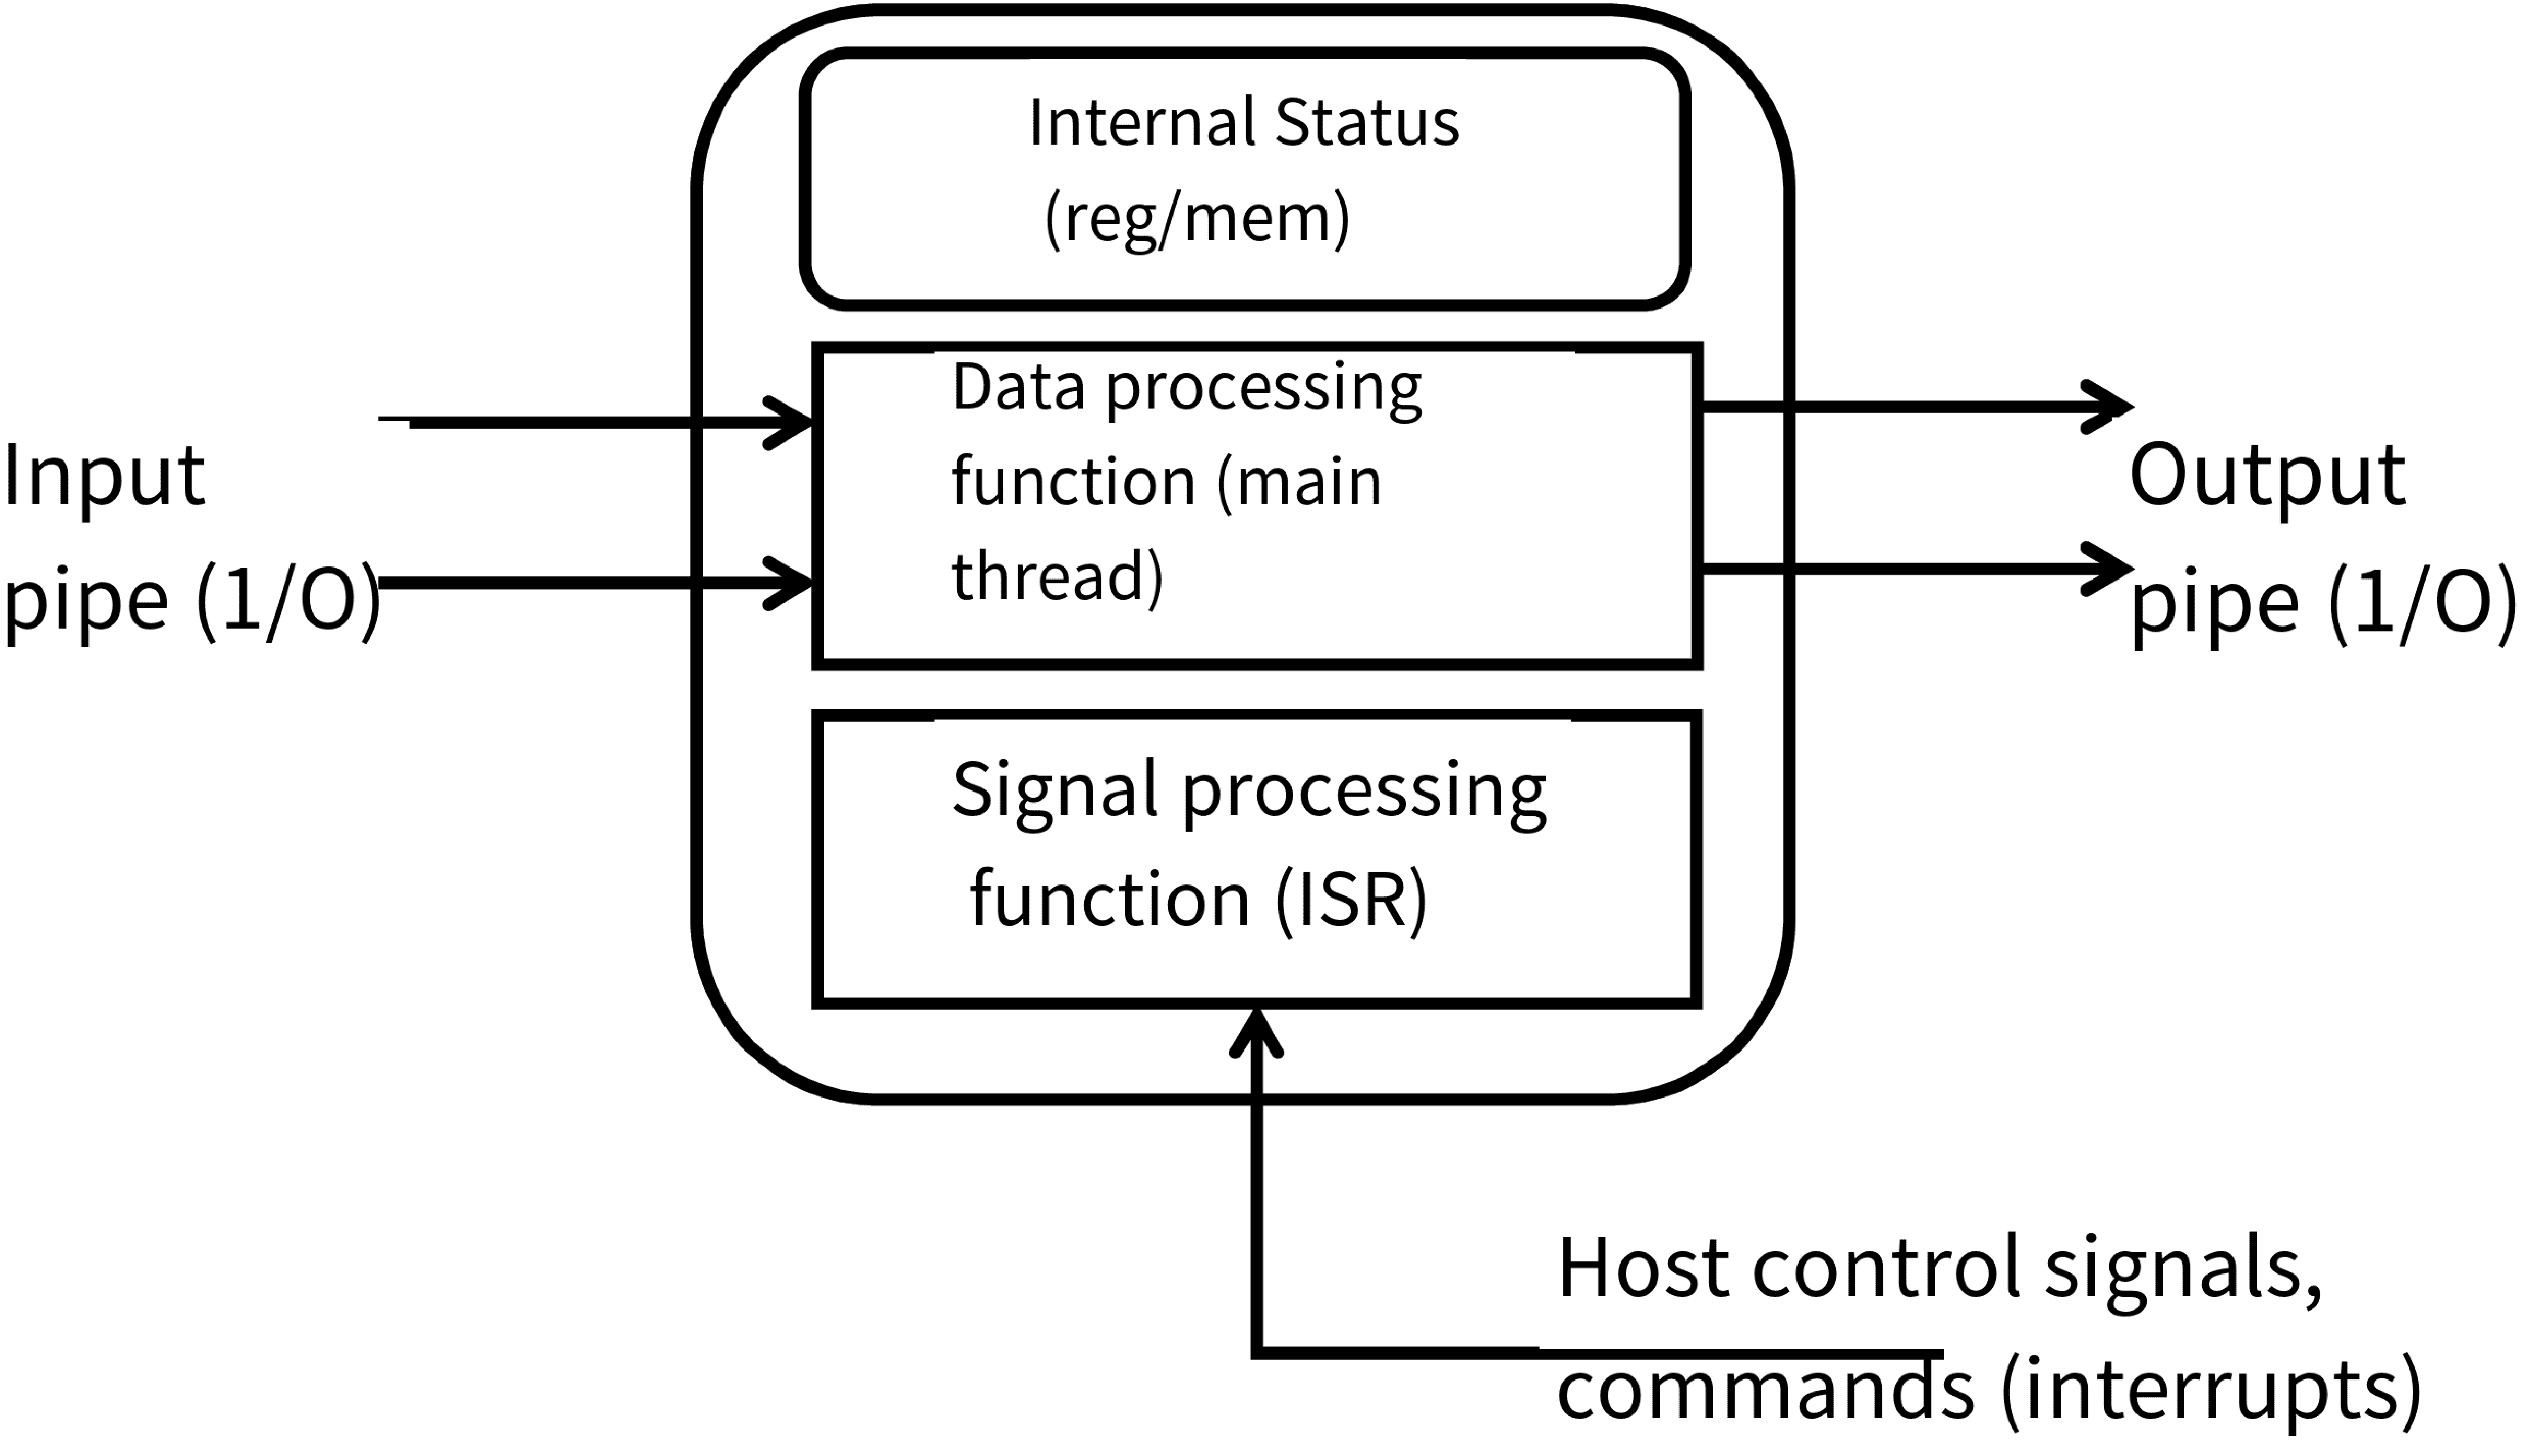
\includegraphics[width=.6\textwidth]{element_arch.pdf}
\caption{ClickNP 元件的构成。}
\label{clicknp:fig:element_arch}
\end{figure}

元件的输出端口可以通过\textit {管道}(channel)连接到另一个元件的输入端口,如图\ref {clicknp:fig:element}(a)所示。
在 \name 中,通道基本上是一个FIFO缓冲区,写入一端并从另一端读取。
对通道的读/写操作的数据单元称为 \textit {flit},其具有64字节的固定大小。
flit的格式如图 \ref {clicknp:fig:element}(b)所示。每个flit包含元数据的标头和32字节的有效负载。
当在 \name 元件之间流动时,大量数据(例如,完整大小的数据包)被分成多个flits。
第一个flit标有 \textbf {sop}(数据包开始),最后一个flit标有 \textbf {eop}(数据包结束)。
如果数据块的大小不是32,则最后一个flit的 \textbf {pad}字段表示已填充到有效负载的字节数。
通过硬件描述语言综合工具优化了flit中的保留字段。
将大数据分解为flits不仅可以减少延迟,还可以在不同元件处同时处理分组的不同片段,以增加并行性。
最后,为了实现网络功能,可以将多个\name 元件互连以形成定向处理图,称为\name \textit {配置}。

\begin{figure}[htbp]
	\centering
	\begin{tabular}{c}
		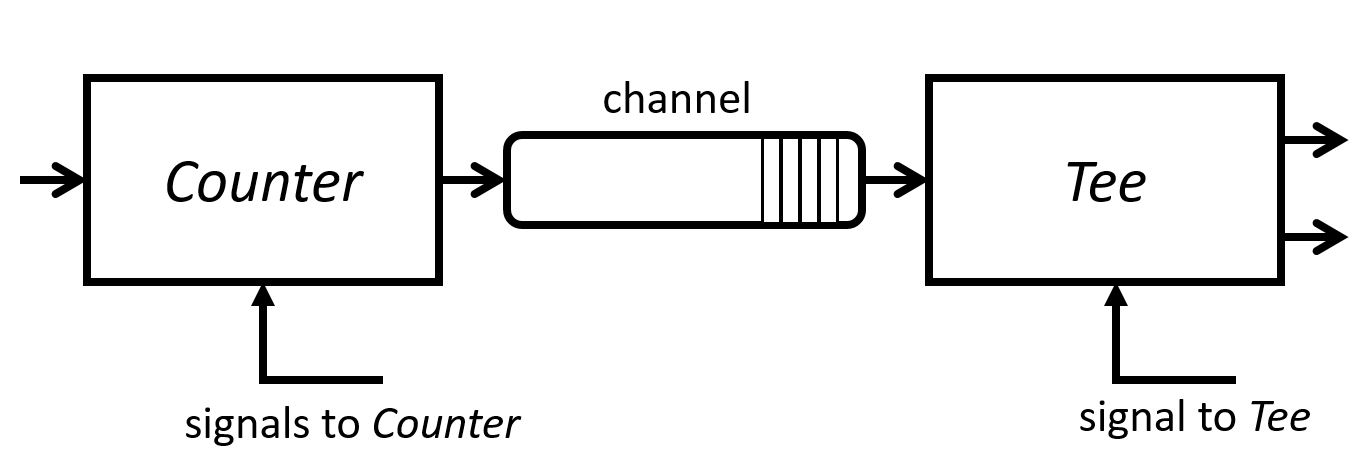
\includegraphics[width=.7\textwidth]{element.jpg}  \\
		(a)\\
		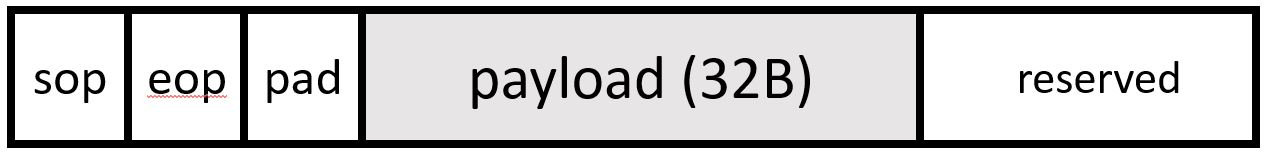
\includegraphics[width=.6\textwidth]{flit.jpg} \\
		(b) \\
	\end{tabular}
	\caption{(a) 两个用管道相连接的 \name 元件。 (b) Flit 的格式。}
	\label{clicknp:fig:element}
\end{figure}


显然,\name 编程抽象很像Click软件路由器 \cite {kohler2000click}。
但是,有三个基本差异使得 \name 更适合FPGA实现:
(1)在Click中,元件之间的边是C ++函数调用,并且需要\textit {queue}元件来存储数据包。
但是,在 \name 中,边实际上表示可以保存实际数据的FIFO缓冲区。此外,\name  channels打破了元件之间的数据依赖关系,并允许它们并行运行。
(2)与Click不同,其中每个输入/输出端口可以是\textit {push或pull},\name 统一了这些操作:一个元件只能\textit {write(push)}到任何输出端口,而 \textit {read(pull)}可以从任何输入端口执行此操作。
(3)Click允许元件直接调用另一个元件的方法(通过基于流的路由器上下文),在 \name 中元件之间的协调是\textit {基于消息},例如,请求者向响应者发送请求消息并通过另一个消息获得响应。
与通过共享内存进行协调相比,基于消息的协调允许更多的并行性并且在FPGA中更有效,其中访问共享内存位置必须被序列化并且将成为瓶颈。

\subsubsection{语言}

\name 元件(element)可以声明为面向对象语言(如 C++)中的一个对象。
不幸的是,许多现有的高层次综合工具仅支持C语言。
为了利用商业高层次综合工具,可以编写一个编译器,将面向对象的语言(例如 C++)转换为C,但这种努力并非易事。
本文采用一种替代路径来扩展C语言以支持元件声明。
图 \ref {clicknp:fig:lang}(a)显示了元件 \textit {Counter}的代码片段,它只计算传递了多少个数据包。元件由 \textbf {.element}关键字定义,后跟元件名称和输入/输出端口数。
关键字 \textbf {.state} 定义元件的状态变量,\textbf {.init},\textbf {.handler} 和 \textbf {.signal}指定初始化,处理和信号处理函数元件。
实现了一组内置函数来对输入和输出端口进行操作,如表 \ref {clicknp:tab:built-in} 中所述。

与Click类似,\name 也使用简单脚本来指定网络功能的配置。配置有两部分:\textit {声明} 和 \textit {连接},遵循Click语言的类似语法 \cite {kohler2000click}。
值得注意的是,在 \name 中,可以使用关键字 \textbf {host}来注释元件,这将导致元件被编译为CPU二进制文件并在CPU上执行。

\iffalse
\textbf{Verilog 元件。}
\fi

\begin{table}

\centering
\caption{\name\ 管道上的内置操作。}
\label{clicknp:tab:built-in}
\scalebox{0.9}{
\begin{tabular}{p{.4\textwidth}|p{.5\textwidth}}
\toprule
uint get\_input\_port() & 获取具有可用数据的所有输入端口的位图。 \\
\midrule
bool test\_input\_port(uint id) & 测试id指示的输入端口。 \\
\midrule
flit read\_input\_port(uint id) & 读取id指示的输入端口。 \\
\midrule
flit peek\_input\_port(uint id) & 获取id指示的输入端口数据,但不取走。 \\
\midrule
void set\_output\_port(uint id, flit x) & 将flit设置为输出端口。 处理程序返回时,flit将写入管道。\\
\midrule
ClSignal read\_signal() & 从信号端口读取信号。\\
\midrule
void set\_signal(ClSignal p) & 在信号端口上设置输出信号。\\
\midrule
return (uint bitmap) & \textbf{.handler} 的返回值指定下一次迭代时要读取的输入端口的位图。 \\
\bottomrule
\end{tabular}
}
\end{table}

\begin{figure}[htbp]
\small \lstset{style=numbers}

\lstset{ emph={%
 element, init, state, handler, signal,include
}, emphstyle={\bfseries .},
morekeywords={get_input_port,read_input_port,from_tor, to_tor, set_output_port, host, set_signal} 
}
\centering
\begin{tabular}{c}
\small
\begin{lstlisting}
element Count <1, 1> {
  state{
    ulong count;
  }
  init{
    count = 0;
  }
  handler{
    if (get_input_port() != PORT_1) {
      return (PORT_1); 
    }
    flit x;
    x = read_input_port(PORT_1);
    if (x.fd.sop) count = count + 1;
    set_output_port(PORT_1, x);
   
    return (PORT_1);
  }
  signal{
    ClSignal p;
    p.Sig.LParam[0] = count;
    set_signal(p);
  }
}
\end{lstlisting} \vspace{3pt} \\
{\normalsize \centering (a)} \vspace{3pt} \\
\begin{lstlisting}
Count :: cnt @ 
Tee :: tee 
host PktLogger :: logger

from_tor -> cnt -> tee [1] -> to_tor
tee [2] -> logger
\end{lstlisting} \vspace{3pt} \\
{\normalsize \centering (b)} 
\end{tabular}
\caption{用 \name 语言写入元件并指定配置的示例。 使用 \textbf {host}关键字注释的元件在CPU上编译和执行。 用“@”注释的元件需要从管理器线程接收控制信号。
	\textbf {``From\_tor''} 和 \textbf {``to\_tor''}是两个内置元件,代表FPGA上以太网端口的输入和输出。 处理函数的返回值指定了将在下一轮中检查的输入端口的位掩码。}
\label{clicknp:fig:lang}

\end{figure}

\subsubsection{\name 工具链}
\label{clicknp:subsec:toolchain}
\name 工具链包含一个 \name 编译器作为前端,一个 C / C++ 编译器(例如,Visual Studio或GCC)和一个高层次综合工具(例如,Altera OpenCL SDK或Xilinx Vivado 高层次综合)作为后端。
如图\ref{clicknp:fig:clicknp}所示,要编写 \name 程序,开发人员需要将代码分为三部分:
(1)一组元件,每个元件实现概念上简单的操作,
(2)指定这些元件之间连接的配置文件,以及(3)主机管理器,它初始化每个元件并在运行时控制它们的行为,例如,根据管理员的输入。
这三部分源代码被送入 \name 编译器并转换为主程序和FPGA程序的中间源文件。
主程序可以由普通的C / C++编译器直接编译,而FPGA程序则使用商业高层次综合工具合成。
现有的商用高层次综合工具可以通过时序分析确定每个元件的最大时钟频率。
然后,\name 处理图的时钟受到图中最慢元件的约束。
另外,高层次综合工具还可以生成优化报告,该报告显示元件中的操作之间的依赖性。如果解析了所有依赖关系并且元件通过在每个时钟周期中处理一个flit来实现最佳吞吐量,则元件是\textit {完全流水线化}的。
\egg{
Our ClickNP architecture is built on state-of-the-art data center reconfigurable hardware (Catapult FPGA \cite{putnam2014reconfigurable}) and FPGA programming framework (Altera OpenCL \cite{singh2011implementing}).

\subsection{Catapult FPGA}

Catapult \cite {putnam2014reconfigurable}是一个可重新配置的硬件,用于在搜索引擎排名中卸载特征提取,特征计算和评分。本章修改硬件以包含两个板载40 GE MAC,因此FPGA可以通过两个40 GE端口接收和发送网络数据包,而无需CPU干预。

\begin{figure}[!t]
	\center
	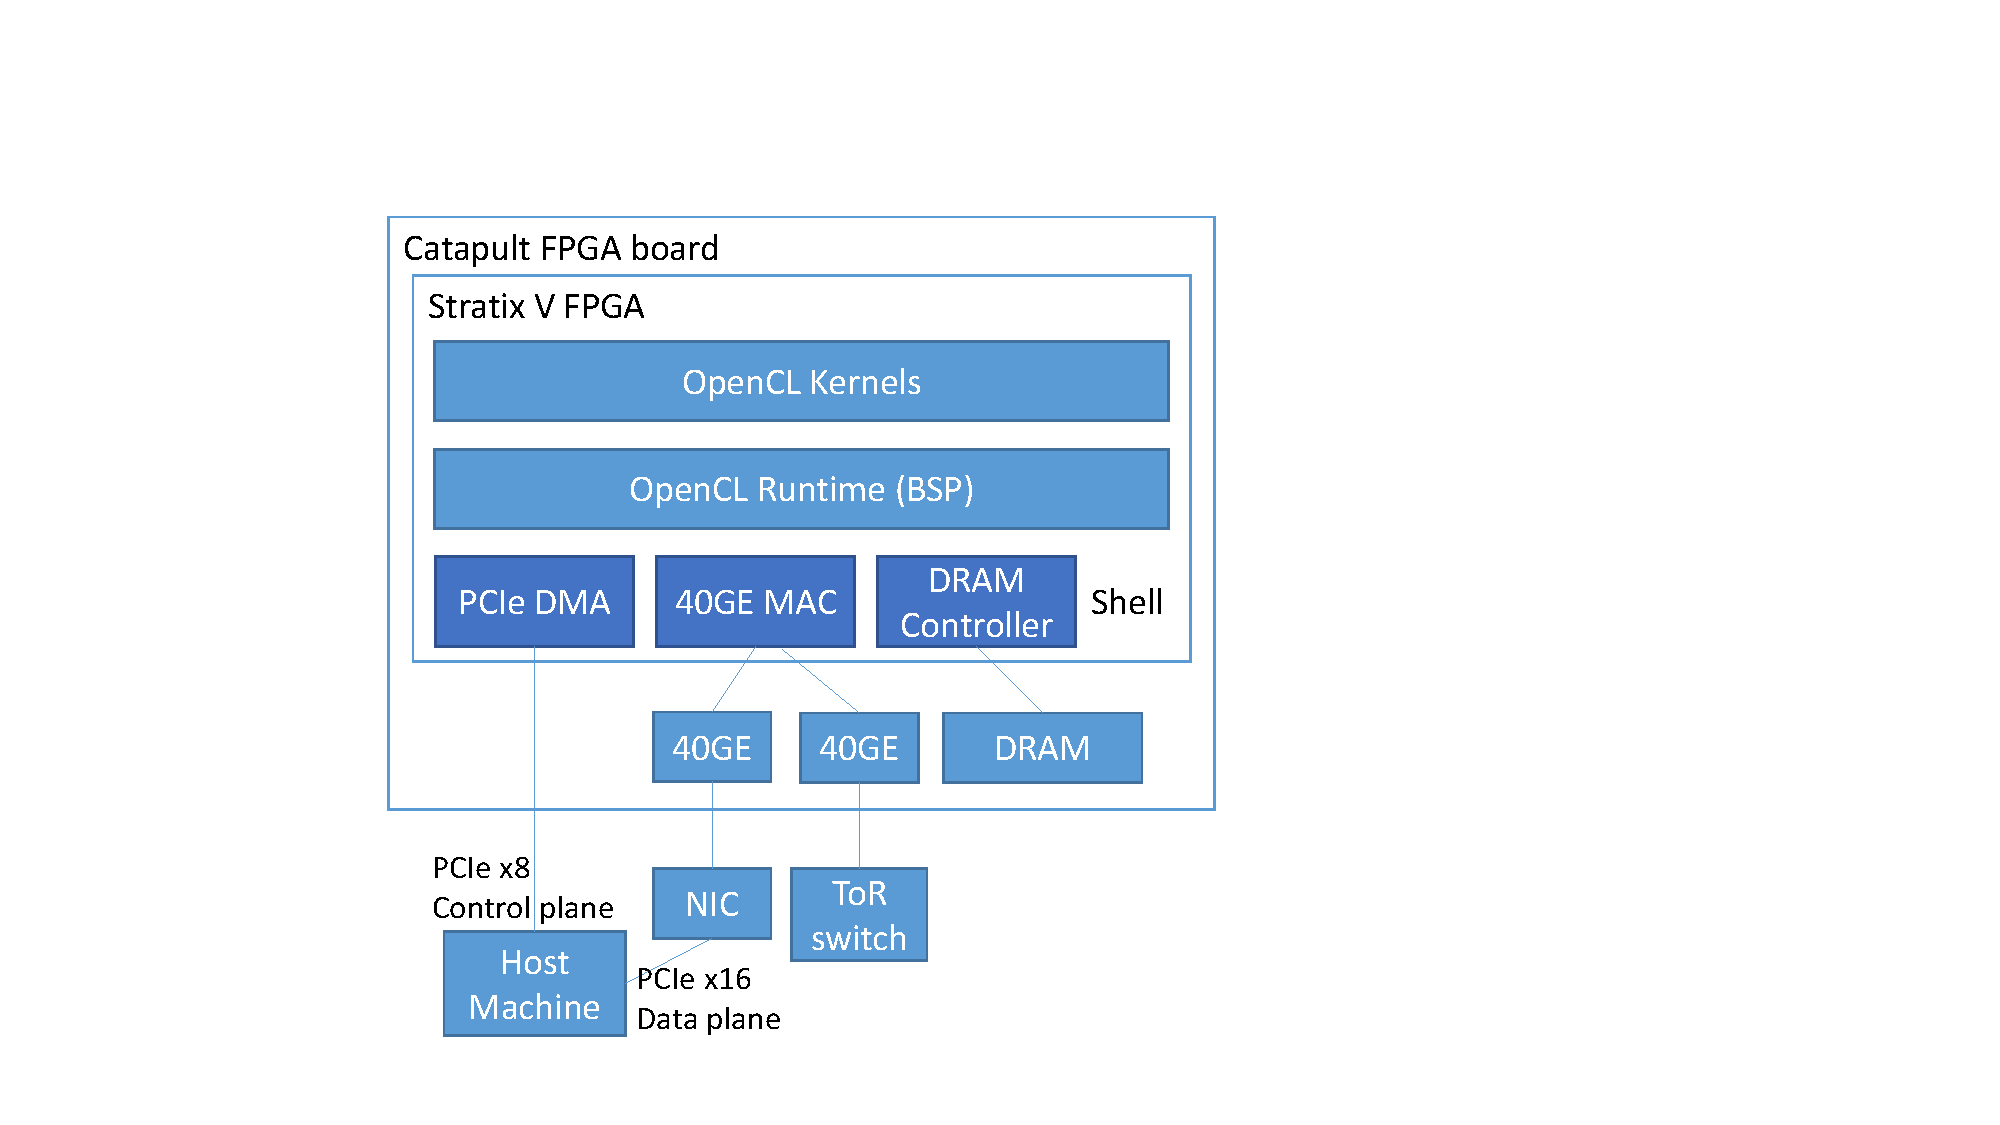
\includegraphics[width=1.0\columnwidth]{image/CatapultFPGAArch}
	\vspace{-0.25in}
	\caption{Catapult FPGA Architecture}
	\vspace{-0.15in}
	\label{clicknp:fig:CatapultFPGAArch}
	%    
\end{figure}

In network virtualization scenario, we install one FPGA in each server and connect two 40 GE ports to 网卡 and Top-of-Rack (ToR) switch respectively. The traffic between 网卡 and ToR flow through the FPGA to perform comprehensive network functions \textit{bump-in-the-wire}, including tunnel encapsulation and decapsulation, firewall, metering and traffic scheduling. Virtual machines expose to the 网卡 and FPGA via Single-Root I/O Virtualization (SR-IOV), and data-plane functions of the virtual switch are offloaded to the FPGA.

Current generation of Catapult FPGA has 172,600 ALMs (Adaptive Logic Modules) each containing several 8-input configurable lookup table, two full adders and four one-bit registers \cite{alterafpgaarch}, 2,014 blocks of 20 Kbit SRAM and a 4 GB DRAM. Each register can be read and written every cycle without latency. Each SRAM block can perform one read or write operation with exactly one cycle latency. The performance of DRAM depends on access pattern. When accessed randomly, each operation takes 170 ns (about 34 cycles); when accessed sequentially, the throughput can reach 4 Gbps. Registers, SRAMs and DRAM form a memory hierarchy where faster memory spaces have lower capacity.

\subsection{OpenCL Compiler}

The Altera SDK for OpenCL \cite{singh2011implementing} is a programming framework that abstract away the traditional hardware FPGA development flow. In the OpenCL \cite{khronos2008opencl} model, data-plane functions are wrapped in \textit{kernels} and compiled into hardware accelerators, and control plane on the host machine communicates with kernels via a standard set of APIs. Altera OpenCL introduces \textit{channels} to allow communication among kernels without host intervention.

Central to Altera OpenCL is a compiler \cite{czajkowski2012opencl} that extracts parallelism in OpenCL kernels and generates Verilog code. A parser based on LLVM first parses OpenCL kernel and produces intermediate representation (IR) consisting of instructions and dependencies between them. Then the IR is optimized via live-variable analysis and generate CDFG (Control Data Flow Graph). Based on CDFG, scheduler determines the required clock cycles of each operation, then sequence the operations into a pipeline, where independent operations are parallelized and dependent operations are pipelined. Finally the compiler links to IP library and generates Verilog 硬件描述语言, as well as a profiling report containing estimated resource utilization and an optimization report containing data dependencies that lead to pipeline stall.

OpenCL is designed primarily for batch processing instead of stream processing, which is a gap that ClickNP needs to bridge. In network stream processing, kernels run in an infinite loop, so the kernels will never finish.

First, when a kernel is running, global memory assigned to it cannot be accessed by the host machine. So commands can not be passed to kernels via global memory on-the-fly. One straightforward approach could be launching another ``proxy'' kernel to pass in commands via channel each time the host sends a command. However, this approach has about 5 millisecond latency due to complicated internals in launching and finishing a kernel. Fortunately, OpenCL only occupies PCIe slots 0--31, so we designed a raw I/O channel via PCIe slots 32--39 to allow on-the-fly interaction of kernels and the host. Figure \ref{clicknp:fig:PCIeChannelPerf} shows that PCIe I/O channels reach near-theoretical throughput with 5 slots and 16K batch size, and the latency for small batch size is microsecond-scale.

\begin{figure}[h!]
	\centering
	\subfigure[Latency (x: batch size, y: microsec; lines: polling, interrupt, opencl)]{
		
\includegraphics[width=0.45\columnwidth]{image/logo}
		\label{clicknp:fig:PCIeChannelLatency}
	}
	\subfigure[Throughput (x : number of slots; y: Gbps; lines: batch size, theory)]{
		
\includegraphics[width=0.45\columnwidth]{image/logo}
		\label{clicknp:fig:PCIeChannelThroughput}
	}
	\vspace{-0.15in}
	\caption{PCIe Channel Performance}
	\vspace{-0.15in}
	\label{clicknp:fig:PCIeChannelPerf}
	%    
\end{figure}

Second, since the kernels never finish, when the host program crashes or need to be updated, although the data plane is still running, we might lose the control plane because the kernels may have problem launching again. We added a PCIe-controlled register to trigger reset signal of OpenCL kernel programs and OpenCL runtime on FPGA. When the host program restarts, it toggles the reset register to force stop all kernels and then re-launch them via OpenCL API.

\subsection{ClickNP Toolchain}

The building blocks of ClickNP are \textit{elements}. Each element is compiled to an OpenCL single-work-item \textit{kernel}.

A ClickNP \textit{project} consists of 3 parts: a library of elements, a \textit{Click script} to specify what and how elements are connected, and a \textit{host program} to interact with the user and issue commands to elements.

ClickNP provides 4 build targets for a project:

\begin{enumerate}
	\item Native x86 emulation (in seconds) with ClickNP compiler and standard C++ compiler to test functionality and debug with \textit{printf}.
	\item Generate optimization report (in 1 minute) to understand resource utilization and memory dependencies with ClickNP compiler and OpenCL compiler. If an element is not fully pipelined, or the overall resource utilization is too high, developer should optimize the element code (if a new element is written) or change element parameters (e.g. lookup table size).
	\item Build full FPGA image (in 1--2 hours) with ClickNP compiler, OpenCL compiler and Quartus synthesizer, fitter, assembler and timing analyzer.
	\item Build host program (in seconds) with ClickNP compiler and standard C++ compiler.
\end{enumerate}

%Multiple emulation-mode ClickNP projects can be connected via named pipes, e.g. connect the traffic generator, your bump-in-the-wire ClickNP project and the traffic monitor with pipes to test functionality with various traffic patterns without code modifications.

\begin{figure}[!t]
	\centering
	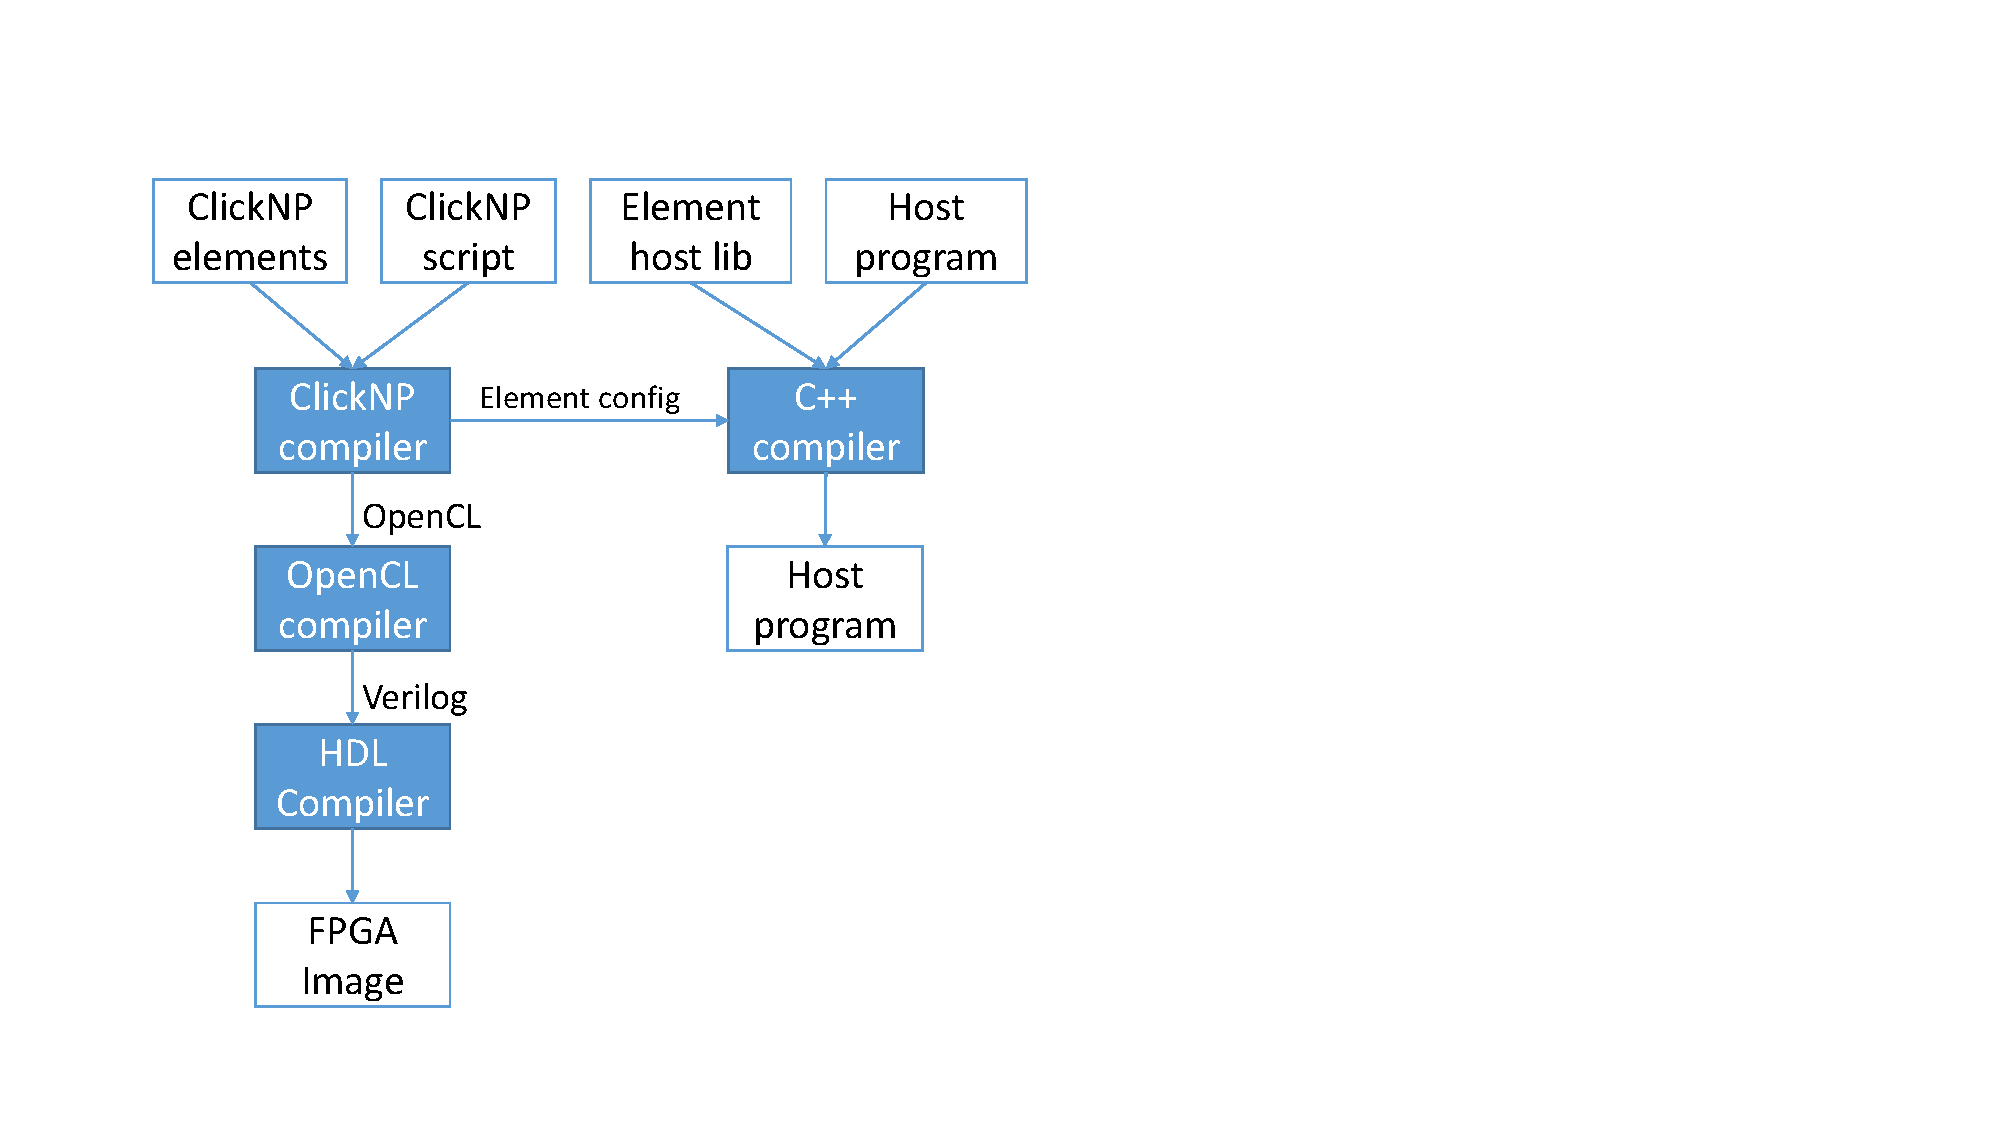
\includegraphics[width=0.8\columnwidth]{image/ClickNPSoftware}
	\vspace{-0.15in}
	\caption{ClickNP Compilation Flow}
	\vspace{-0.15in}
	\label{clicknp:fig:ClickNPSoftware}
	%    
\end{figure}

Full compilation of a project generates an FPGA image, a x86 host program and an OpenCL kernel binary. First, the FPGA image is reprogrammed into FPGA via Flash Util in Figure \ref{clicknp:fig:CatapultFPGAArch} (30 seconds). Second, the host program starts, resets the FPGA board, loads OpenCL kernel binary and launches all kernels. Then the host program keeps running, accepts control plane commands via terminal or RPC, issues signals to elements and listen to events from elements.

When the host program needs to be updated, simply kill the host program and the data plane will keep running. The new host program can choose to either re-initialize all element states, or keep the states and clear in-flight signals and events in case the host program was killed halfway in host-kernel communication.

\begin{figure}[!t]
	\centering
	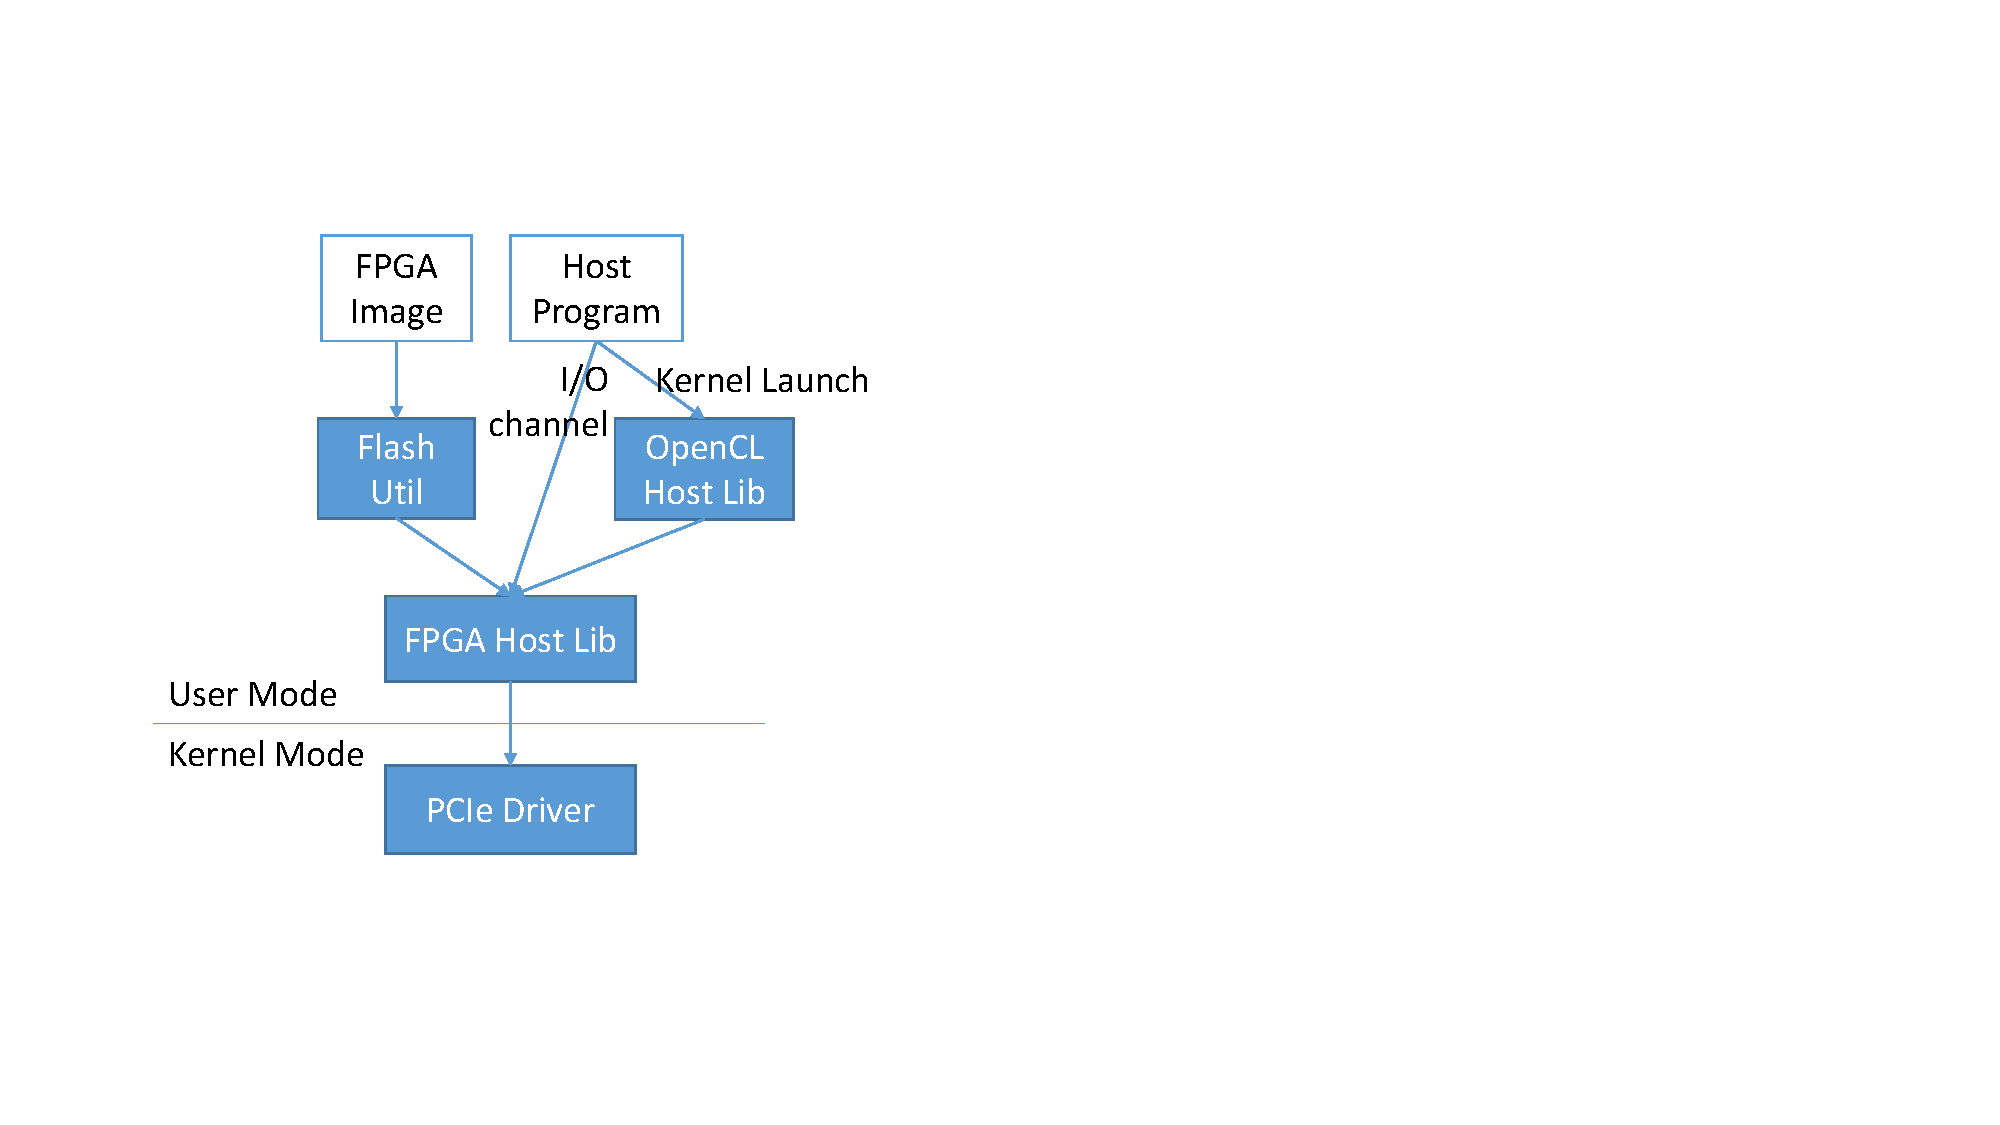
\includegraphics[width=0.8\columnwidth]{image/CatapultRuntime}
	\vspace{-0.15in}
	\caption{ClickNP Runtime Architecture}
	\vspace{-0.15in}
	\label{clicknp:fig:CatapultFPGAArch}
	%    
\end{figure}
}
